\chapter{研究内容2}
\thispagestyle{mainstyle} % \chapter后面必须加这条命令启动页眉页脚设置
\section{介绍}
介绍。介绍。介绍。介绍。介绍。介绍。

介绍。介绍。介绍。介绍。介绍。介绍。

介绍。介绍。介绍。介绍。介绍。介绍。

\section{相关工作}
相关工作。相关工作。相关工作。相关工作。

相关工作。相关工作。相关工作。相关工作。

\section{方法}
方法。方法。方法。方法。方法。方法。方法。

方法。方法。方法。方法。方法。方法。方法。

公式\ref{eq:eq2}。

\begin{equation}
    a^2 + b^2 = c^2 \label{eq:eq2}
\end{equation}

图片\ref{fig:image2}。
\begin{figure}
    \centering
    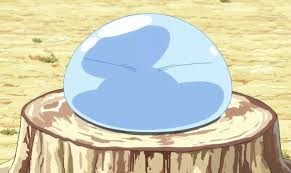
\includegraphics[width=0.8\textwidth]{images/image.jpeg}
    \caption{××图}
    \label{fig:image2}
\end{figure}

表格\ref{tab:table2}。
\begin{table}
    \centering
    \caption{**表}
    \label{tab:table2}
    \begin{tabular}{c|c}
        \toprule[1.5bp]
        列1 & 列2 \\
        \midrule[0.75bp]
        值1 & 值2 \\
        值1 & 值2 \\
        \bottomrule[1.5bp]
    \end{tabular}
\end{table}

\section{实验}
实验。实验。实验。实验。实验。

实验。实验。实验。实验。实验。